\documentclass{article}\usepackage[]{graphicx}\usepackage[]{xcolor}
% maxwidth is the original width if it is less than linewidth
% otherwise use linewidth (to make sure the graphics do not exceed the margin)
\makeatletter
\def\maxwidth{ %
  \ifdim\Gin@nat@width>\linewidth
    \linewidth
  \else
    \Gin@nat@width
  \fi
}
\makeatother

\definecolor{fgcolor}{rgb}{0.345, 0.345, 0.345}
\newcommand{\hlnum}[1]{\textcolor[rgb]{0.686,0.059,0.569}{#1}}%
\newcommand{\hlsng}[1]{\textcolor[rgb]{0.192,0.494,0.8}{#1}}%
\newcommand{\hlcom}[1]{\textcolor[rgb]{0.678,0.584,0.686}{\textit{#1}}}%
\newcommand{\hlopt}[1]{\textcolor[rgb]{0,0,0}{#1}}%
\newcommand{\hldef}[1]{\textcolor[rgb]{0.345,0.345,0.345}{#1}}%
\newcommand{\hlkwa}[1]{\textcolor[rgb]{0.161,0.373,0.58}{\textbf{#1}}}%
\newcommand{\hlkwb}[1]{\textcolor[rgb]{0.69,0.353,0.396}{#1}}%
\newcommand{\hlkwc}[1]{\textcolor[rgb]{0.333,0.667,0.333}{#1}}%
\newcommand{\hlkwd}[1]{\textcolor[rgb]{0.737,0.353,0.396}{\textbf{#1}}}%
\let\hlipl\hlkwb

\usepackage{framed}
\makeatletter
\newenvironment{kframe}{%
 \def\at@end@of@kframe{}%
 \ifinner\ifhmode%
  \def\at@end@of@kframe{\end{minipage}}%
  \begin{minipage}{\columnwidth}%
 \fi\fi%
 \def\FrameCommand##1{\hskip\@totalleftmargin \hskip-\fboxsep
 \colorbox{shadecolor}{##1}\hskip-\fboxsep
     % There is no \\@totalrightmargin, so:
     \hskip-\linewidth \hskip-\@totalleftmargin \hskip\columnwidth}%
 \MakeFramed {\advance\hsize-\width
   \@totalleftmargin\z@ \linewidth\hsize
   \@setminipage}}%
 {\par\unskip\endMakeFramed%
 \at@end@of@kframe}
\makeatother

\definecolor{shadecolor}{rgb}{.97, .97, .97}
\definecolor{messagecolor}{rgb}{0, 0, 0}
\definecolor{warningcolor}{rgb}{1, 0, 1}
\definecolor{errorcolor}{rgb}{1, 0, 0}
\newenvironment{knitrout}{}{} % an empty environment to be redefined in TeX

\usepackage{alltt}
\usepackage{amsmath} %This allows me to use the align functionality.
                     %If you find yourself trying to replicate
                     %something you found online, ensure you're
                     %loading the necessary packages!
\usepackage{amsfonts}%Math font
\usepackage{graphicx}%For including graphics
\usepackage{hyperref}%For Hyperlinks
\usepackage[shortlabels]{enumitem}% For enumerated lists with labels specified
                                  % We had to run tlmgr_install("enumitem") in R
\hypersetup{colorlinks = true,citecolor=black} %set citations to have black (not green) color
\usepackage{natbib}        %For the bibliography
\setlength{\bibsep}{0pt plus 0.3ex}
\bibliographystyle{apalike}%For the bibliography
\usepackage[margin=0.50in]{geometry}
\usepackage{float}
\usepackage{multicol}

%fix for figures
\usepackage{caption}
\newenvironment{Figure}
  {\par\medskip\noindent\minipage{\linewidth}}
  {\endminipage\par\medskip}
\IfFileExists{upquote.sty}{\usepackage{upquote}}{}
\begin{document}

\vspace{-1in}
\title{Lab 10 -- MATH 240 -- Computational Statistics}

\author{
  Pierce Leclerc \\
  Colgate University  \\
  Department of Mathematics  \\
  {\tt pleclerc@colgate.edu}
}

\date{}

\maketitle

\begin{multicols}{2}
%\raggedcolumns % If your spacing gets messed up try uncommenting 
                % this line
\begin{abstract}
We examine the effect of sample size and assumed true probability on margin of error. Data from Gallup is compared to random samples, and margins of errors of both are compared as well. Resampling is performed on the Gallup data to estimate margin of error. Margin of error is plotted as a function of $n$ and $p$ to demonstrate the pairs which maximize it, and these conclusions are verified by comparison to the Wilson Estimates.
\end{abstract}

\noindent \textbf{Keywords:} Margins of Error, Resampling, Simulation

\section{Introduction}
In Lab 10, we look to examine the effect that sample size and actual population proportion have on margin of error. Gallup reports that a sample size of 1000 national adults corresponds to accuracy with a margin of error of $\pm 4\%$, while doubling the sample size decreases the margin of error to $\pm 2\%$. Under an assumed true probability, we conduct a sample simulation study to determine margin of error under sample sizes of 1000 and 2000 to compare with Gallup's measurements. We then perform resampling on the Gallup data and conduct the same analyses. We perform 10,000 simulations under different values of n and p to observe the effects of both on margin of error and calculate the actual margin of error for verification.

\section{Simulation Studies}

Figures 1 and 2 illustrate the results of 10,000 generated polls of their respective sample sizes. They both appear approximately normally distributed.

\begin{Figure}
\begin{center}
  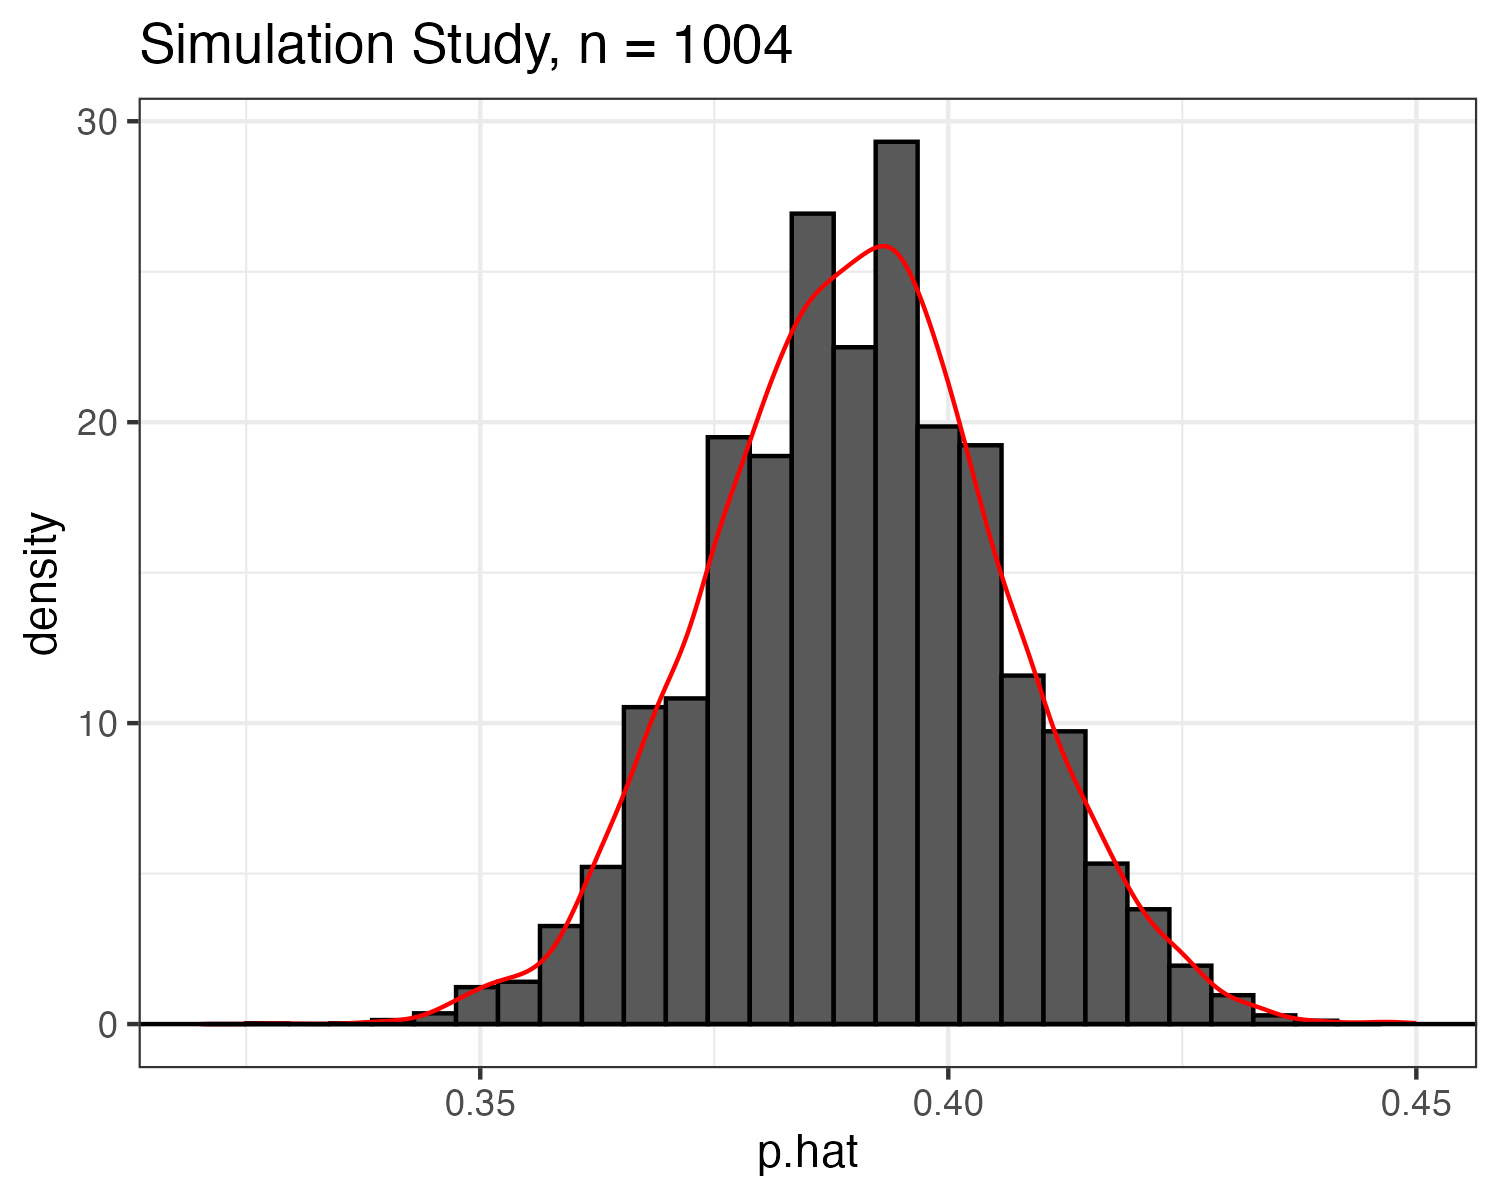
\includegraphics[width=\textwidth]{task1_1.png}
\end{center} 
\captionof{figure}{Simulation study with true probability 0.39 and n = 1004. Density superimposed in red.}
\end{Figure}

With n = 1004, the margin of error is $0.02988048$, or approximately $2.99\%$, slightly less than the $4\%$ reported by Gallup.

\begin{Figure}
\begin{center}
  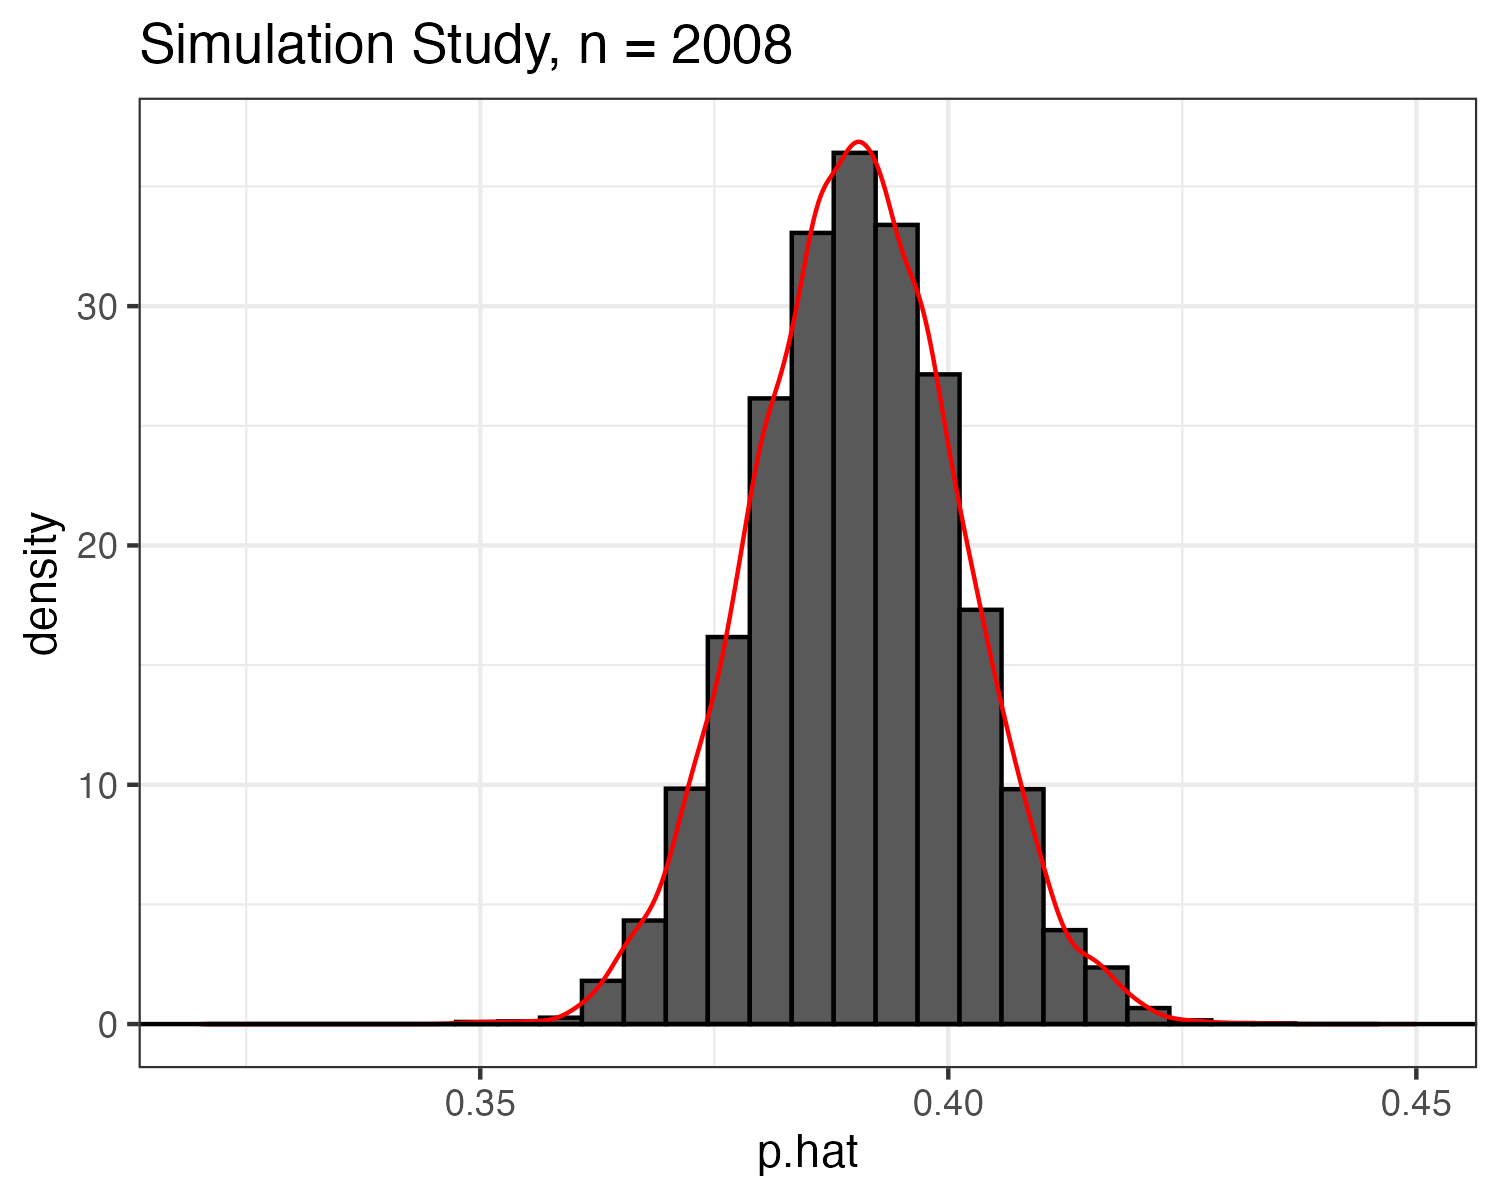
\includegraphics[width=\textwidth]{task1_2.png}
\end{center} 
\captionof{figure}{Simulation study with true probability 0.39 and n = 2008. Density superimposed in red.}
\end{Figure}

With n = 2008, the margin of error is $0.02116534$, or approximately $2.12\%$, similar to the estimate from Gallup of $2\%$.

\section{Resampling}

With sample data from the Gallup survey, resampling was performed and results are plotted in Figure 3. The data appears to be normally distributed once again, but with a mean below the previously assumed true probability of 0.39.

\begin{Figure}
\begin{center}
  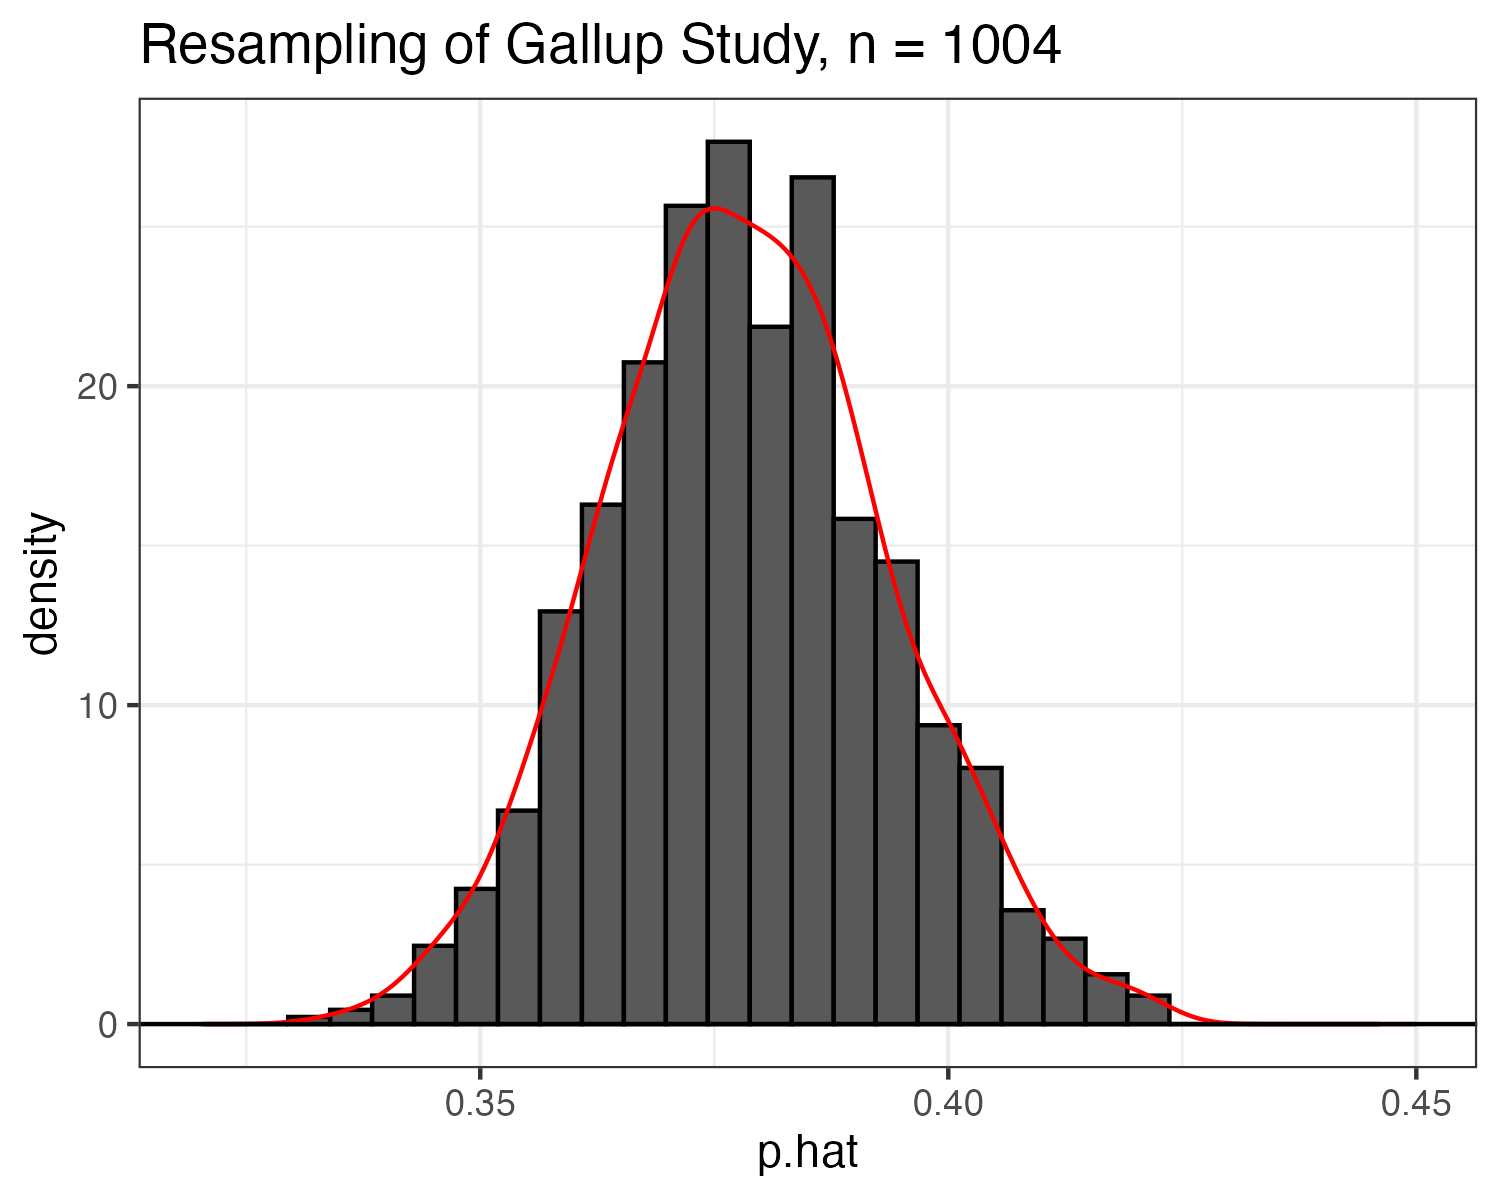
\includegraphics[width=\textwidth]{task2.png}
\end{center} 
\captionof{figure}{Histogram of resampled Gallup data (n = 1004) with density superimposed in red.}
\end{Figure}

The margin of error in this case is $0.02889691$, or approximately $2.89\%$, less than the reported estimate of $4\%$ by Gallup.

\section{Simulation over $n$ and $p$}

10,000 simulations were performed under different values of $n$ and $p$ and are plotted in Figure 4.

\begin{Figure}
\begin{center}
  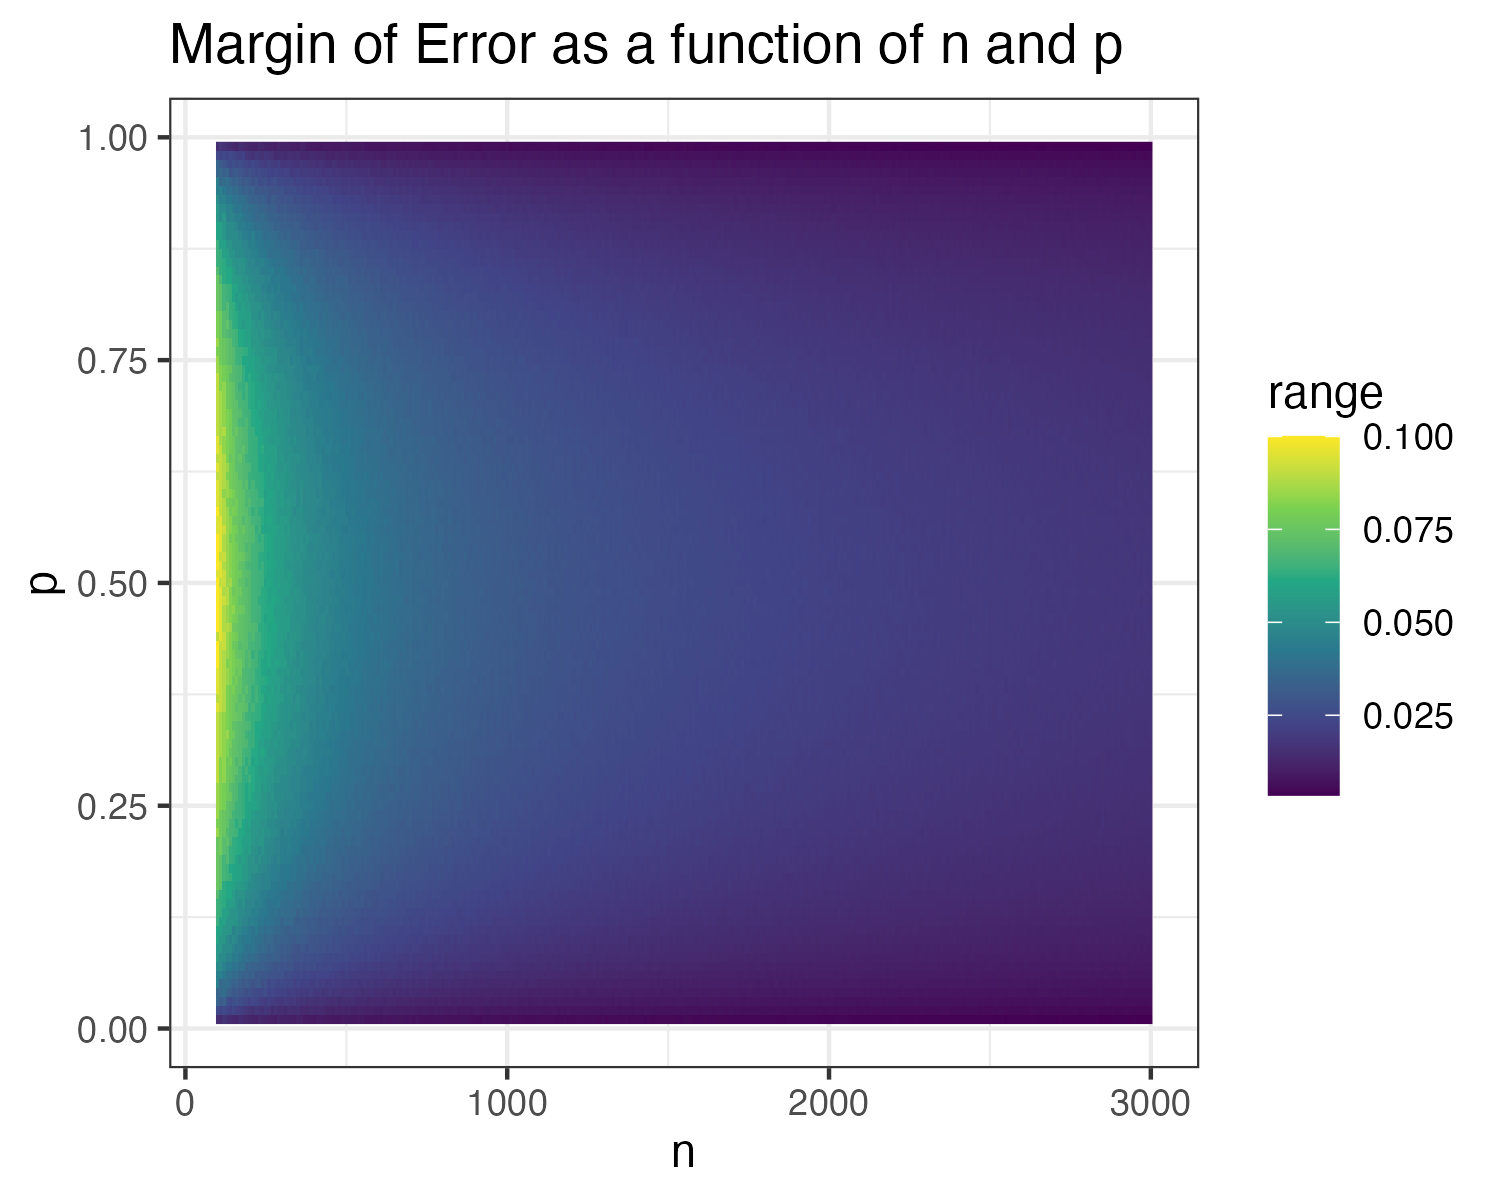
\includegraphics[width=\textwidth]{task3.png}
\end{center} 
\captionof{figure}{Raster plot of estimated margin of error as a function of $n$ and $p$.}
\end{Figure}

From this analysis, it is evident that margin of error is maximized when the sample size is small and the assumed true probability is near $50\%$. To verify this, we compute the actual margins of error via the Wilson Estimate, as shown in figure 5:

\begin{Figure}
\begin{center}
  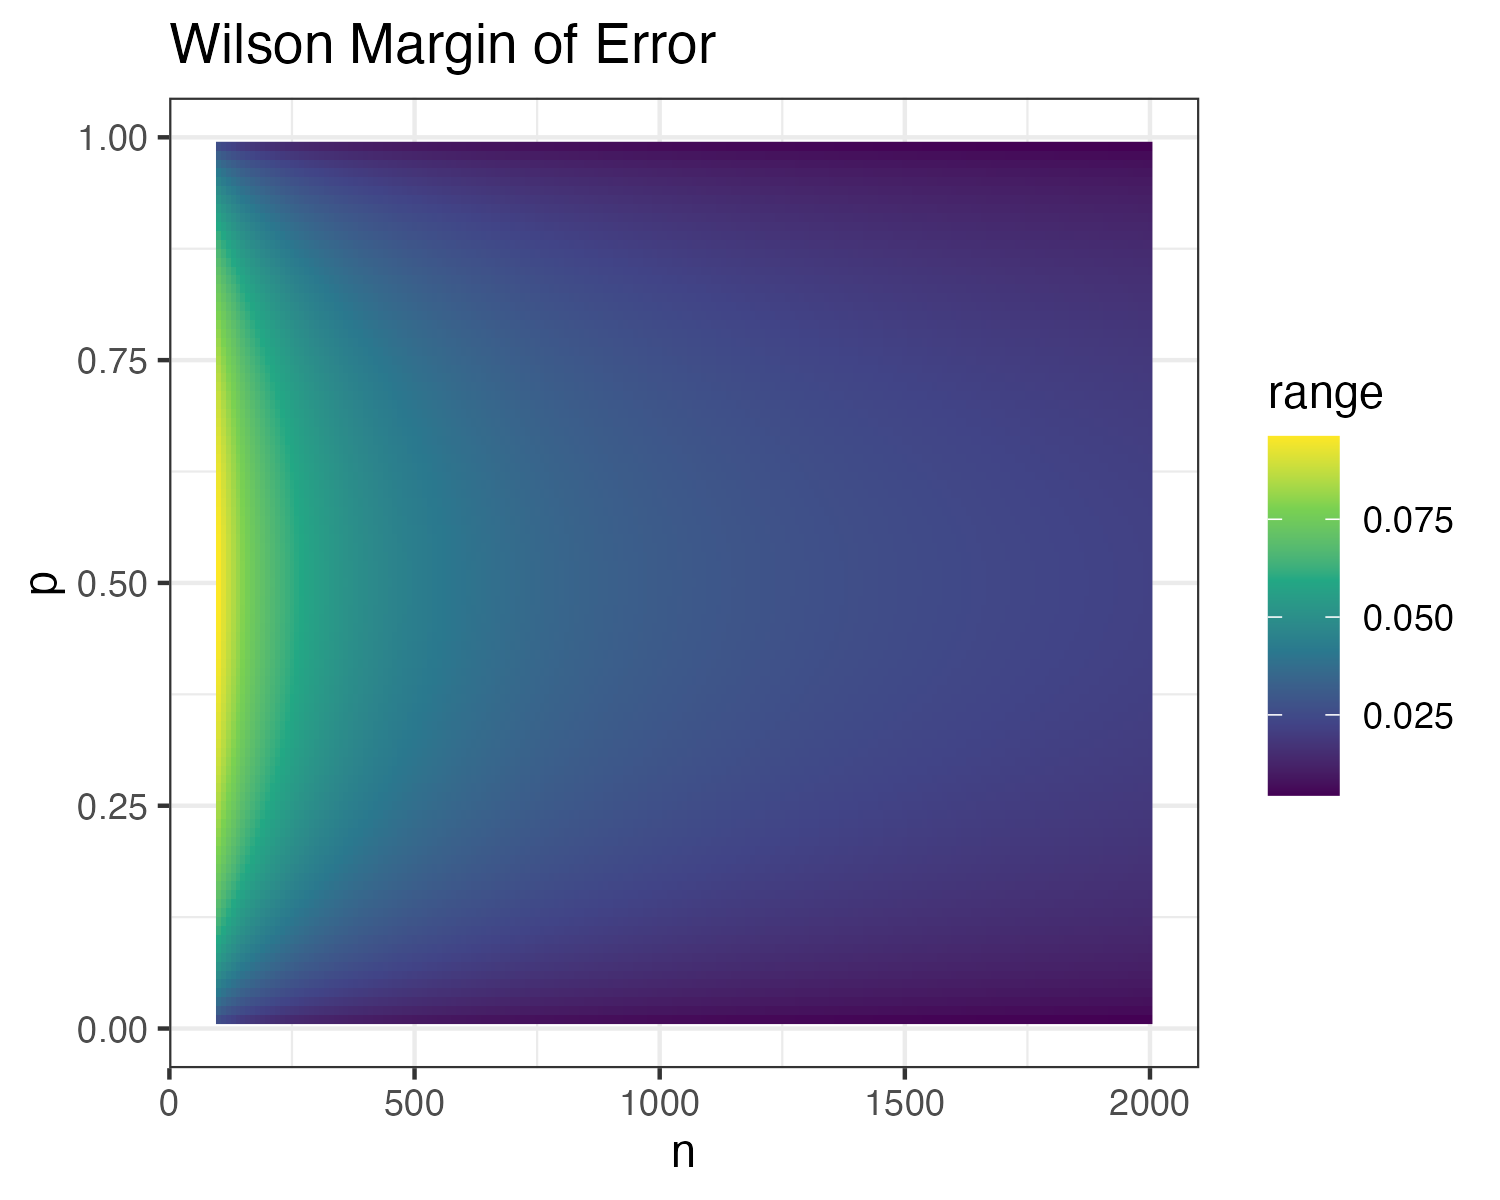
\includegraphics[width=\textwidth]{task4.png}
\end{center} 
\captionof{figure}{Wilson Margin of Error as a function of $n$ and $p$.}
\end{Figure}

%%%%%%%%%%%%%%%%%%%%%%%%%%%%%%%%%%%%%%%%%%%%%%%%%%%%%%%%%%%%%%%%%%%%%%%%%%%%%%%%
% Bibliography
%%%%%%%%%%%%%%%%%%%%%%%%%%%%%%%%%%%%%%%%%%%%%%%%%%%%%%%%%%%%%%%%%%%%%%%%%%%%%%%%
\vspace{2em}

\begin{tiny}
\bibliography{bib}
\end{tiny}
\end{multicols}

%%%%%%%%%%%%%%%%%%%%%%%%%%%%%%%%%%%%%%%%%%%%%%%%%%%%%%%%%%%%%%%%%%%%%%%%%%%%%%%%
% Appendix
%%%%%%%%%%%%%%%%%%%%%%%%%%%%%%%%%%%%%%%%%%%%%%%%%%%%%%%%%%%%%%%%%%%%%%%%%%%%%%%%
\newpage
\onecolumn

\end{document}
